\chapter{Mathematical Background}

The purpose of this chapter is to remind the reader basic notions regarding algebra and statistics, but also to analyze in detail concepts and algorithms concerning lattices, especially integer lattices. 

\section {Algebra}
The notions of group, cyclic group, ring and polynomial are considered to be previously known by the average reader. More information about the mentioned structures can be found in \cite{HPS08}, chapter 2. For a mathematical perspective over groups and polynomial rings properties, and also for a deep incursion in field extension theory, the reader can explore \cite{BB15}.

\begin{enumerate}
	\item \textbf{Ideals and Quotient Rings.} 
	
	\textbf{Definition 5.} \textit{Let $(R, +, \cdot)$ be a commutative finite ring. An \textbf{ideal} of $R$ is a nonempty set $\ci \subseteq R$ that is closed under addition and $ax=xa \in \ci, \forall x \in \ci, \forall a \in R.$} \\
	
	Let $(R, +, \cdot)$ be a finite ring and $\ci$ be an ideal of $R$. Also, let $"\sim"$ be an equivalence relationship on $R$, defined by $x \sim y \iff \exists a\in \ci $ such that $x = y + a$. The equivalence class of an element $x \in R$ is usually noted with $\hat{x}$, and it represents the set $\{y \in R : y \sim x\}$. The equivalence classes generate a partition of the set $R$, named \textit{quotient set}, and denoted by $R/\ci$. It is known that $(R/\ci, +, \cdot)$ is also a ring, and it is called the \textbf{quotient ring} $R/\ci$.
	
	\textbf{Remark 3.} \textit{An example of a quotient ring is the well-known ring $\bZ_p = \bZ/p\bZ.$}
	
	\item \textbf{Cyclotomic polynomials.}
	
	\textbf{Definition 6 \cite{BB15}.} \textit{Let $n \geq 1$ be an integer and $P_n $ be the set of all the $n^{th}$ primitive roots of unity. Then, the \textbf{$n^{th}$ cyclotomic polynomial} is $\Phi_n = \displaystyle{\prod_{\xi \in P_n}}(X-\xi)$}.
	
	\textbf{Remark 4.} Using the fact that $\Phi_{p^k}(X) = \Phi_p(X^{p^{k-1}})$, for any positive integers $k, p$, with $p-$prime, it can be proved that $\Phi_{2^k}(X) = X^{2^{k-1}} + 1,$ for any integer $k \geq 1$.
	
	\item \textbf{Vector spaces}.
	
	Throughout the paper, vectors and matrices are thickened, e.g. $\textbf{v}$. Also, every vector space is considered to be contained in $R^m$, with $m \geq 1$, integer.\\
	
	\textbf{Definition 7 \cite{HPS08}.} \textit{Let $m$ be a positive integer. A \textbf{vector space} $V$ is a subset of $\bR^m$, such that for every $\alpha_1, \alpha_2 \in \bR$ and every} $\textbf{v}_1, \textbf{v}_2 \in V$, it holds: $\alpha_1 \vv_1 + \alpha_2 \vv_2\in V$.
	
	The lecturer is expected to master the concepts of \textit{linear combination, linear independence, basis, vector orthogonality, basis orthogonality}. For a quick review over the mentioned concepts, visit \cite{HPS08}.\\
	
	The only algorithm regarding vector spaces to be presented in the current paper is the  \textbf{Gram-Schmidt Algorithm}. It receives as input a basis $\{\vv_1, .., \vv_n\}$ of the vector space $V$ and outputs $\{\vv_1^*,..,\vv_n^*\}$ - an orthonormal basis of $V$. The algorithm is presented below:

\begin{tcolorbox}[colframe=black,colback=white,arc=0pt,outer arc=0pt]
	\begin{center}
		\textbf{The Gram-Schmidt Algorithm}
	\end{center}
	\begin{algorithmic}[1]
		\State Set $\vv_1^* = \vv_1$
		\For{$i \la 2$ \textbf{to} $n$}
		\State Compute $\mu_{ij} = \vv_i \cdot \vv_j^*$ $/$ $ ||\vv_j^*||$,  for $1 \leq j < i$
		\State Set $\vv_i^* = \vv_i - \displaystyle{\sum_{j = 1}^{i-1}} \mu_{ij} \vv_j^* $
		\EndFor
	\end{algorithmic}
\end{tcolorbox}

	Intuitively, $\mu_{ij}$ represents the length of the projection of $\vv_i$ over $\vv_j^*$. Therefore, the substraction $\vv_i - \mu_{ij} \vv_j^*$ generate the projection of $\vv_i$ over the orthogonal complement of $\vv_j^*$, which leads to the desired output. 
\end{enumerate}	

\section{Lattices}

\subsection{General Influence}

Lattices have been studied by mathematicians such as Gauss, Lagrange or Minkowski since 18$^{th}$ century, and have been used to prove theorems in number theory and the field extensions. Even though lattices confirmed their significance in mathematics, they were not used in computer science until the 1980s, when Lenstra, Lenstra and Lov\`{a}sz proposed the basis-reduction algorithm \textbf{LLL}. It represented a major breakthrough in cryptography, and was used to break several cryptosystems, such as RSA (in a low exponent setting) and NTRU. \\

Since the proposal of \textbf{LLL} algorithm, lattices became appealing to the world of cryptography. Thus, since then they have been used in the construction of cryptographic schemes, such as Attribute Based Encryption \cite{Boy13}, Fully homomorphic encryption \cite{Gen09} and Graded Encoding Systems \cite{GGH13}.

\subsection{Basic Concepts}

\textbf{Definition 8 (\cite{HPS08}).} \textit{Let $n, m$ be two positive integers and let} $B = \{\vv_1, .., \vv_n\} \subset \bR^m$ \textit{ be a set of linearly independent vectors. The \textbf{lattice} generated by $B$ is the set:}
\begin{center}
	$L$   $  \stackrel{\mathclap{\normalfont\mbox{not.}}}{=} \mathcal{L}(B) = \{a_1\vv_1 + a_2 \vv_2 +... + a_n\vv_n : a_1, a_2, ..,a_n \in \bZ\}$.
\end{center}

\textit{Also, a lattice that contains only vectors with integer coordinates is called an \textbf{integer lattice}}. The \textbf{dual lattice} is denoted by $L^* = \{\textbf{y} \in Span(L) : \forall \textbf{x} \in L, \langle\textbf{x, y}\rangle \in \bZ\}$.


From a visual point of view, the elements of a lattice are structured as a net, with massive holes between the nodes, as it can be noticed in Figure 1.

\textbf{Definition 9 (\cite{HPS08}).} \textit{Let $L$ be a $n$-dimensional lattice and} $B = \{\vv_1,...,\vv_n\}$ \textit{be a basis for the lattice $L$. The \textbf{fundamental domain} for $L$ that is associated with $B$ is:}
\begin{center}
	$\mathcal{F}(\vv_1,...,\vv_n) = \{t_1\vv_1 + ...+ t_n\vv_n : t_i \in [0, 1], \forall i \in \{1,..., n\}\}$.
\end{center}


\begin{center}
	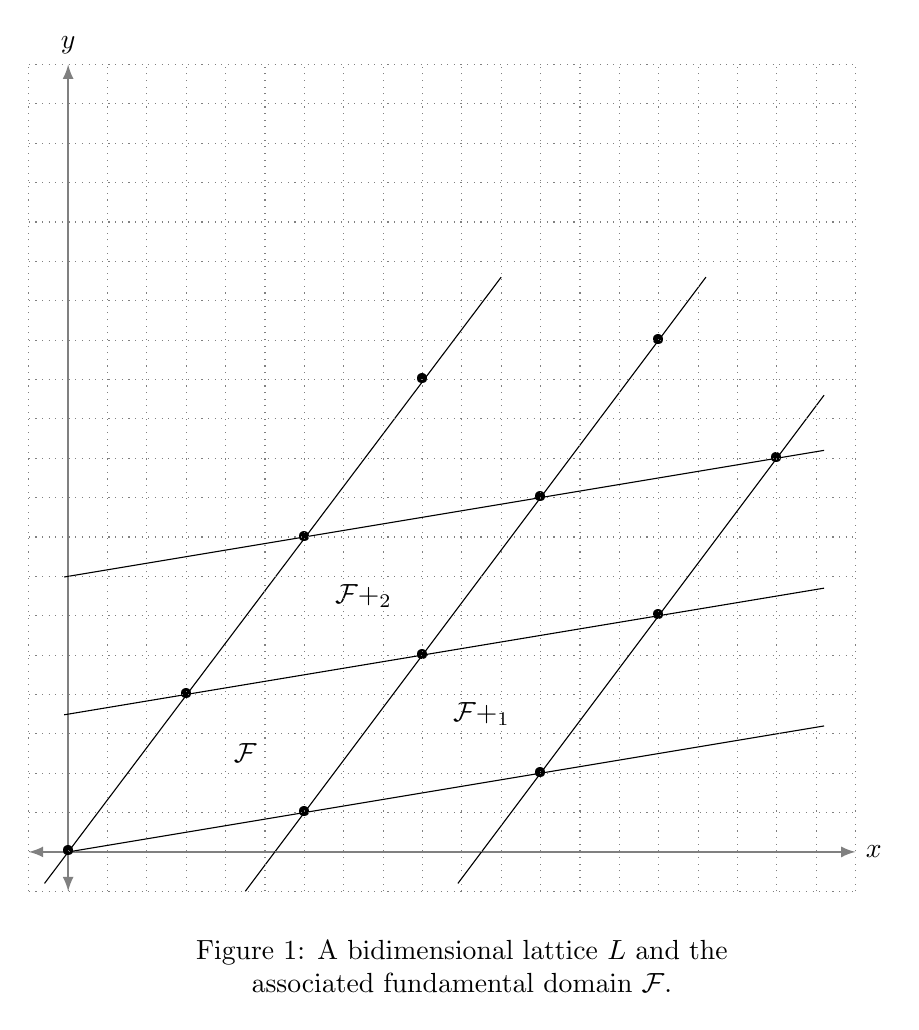
\begin{tikzpicture}[scale = 0.5]
\draw[latex-latex, thick, draw=gray] (-1,0)--(20,0) node [right] {$x$}; 
\draw[latex-latex,thick, draw=gray] (0,-1)--(0,20) node [above] {$y$};

\foreach \Point in {(0, 0), (3, 4), (6,1), (9, 5), (6, 8), (9, 12), (12, 9), (15, 13), (12,2), (15, 6), (18, 10)}{
	\node at \Point {\textbullet};
}

\draw[black] (-0.6, -0.8) -- (11, 14.6);
\draw[black] (4.5, -1) -- (16.2, 14.6);
\draw[black] (9.9, -0.8) -- (19.2, 11.6);

\draw[black] (-0.1, -0.0166) -- (19.2, 3.2);
\draw[black] (-0.1, 3.483333) -- (19.2, 6.7);
\draw[black] (-0.1, 6.983333) -- (19.2, 10.2);


\node [black] at (4.5,2.5) {$\mathcal{F}$};
\node [black] at (10.5,3.5) {$\mathcal{F}+ \vv_1$};
\node [black] at (7.5,6.5) {$\mathcal{F}+ \vv_2$};
\draw [dotted, gray] (-1,-1) grid (20,20);

\node [below=1cm, align=flush center,text width=8cm] at (10, 0)
{
	Figure 1: A bidimensional lattice $L$ and the associated fundamental domain $\mathcal{F}$.
};
\end{tikzpicture}
\end{center}

\textbf{Proposition 2.} \textit{Let $n$ be a positive integer and $L \subset \bR^n$ be a lattice of dimension $n$. Then, for every basis $B$ of $L$, the volume of the fundamental domain associated with it is the same.}\\

\textbf{Definition 10.} \textit{Let $n$ be a positive integer and let $L \subset \bR^n$ be a lattice of dimension $n$. The \textbf{determinant} of $L$ is the volume of any fundamental domain for $L$, and it is denoted by det($L$).}

\textbf{Definition 11.} \textit{Let $i$ be an integer, $i \geq 2$. Also, let $n$ be a positive integer, let $L \subset \bR^n$ be a lattice of dimension $n$ and let $B$ be a basis of $L$. Then, the $i^{th}$ \textbf{successive minimum} is the smallest $r$ such that $rB$ contains $i$ linearly independent lattice points}, and is denoted by:
\begin{center}
	$\lambda_i(L) = \displaystyle{\min}\{r:\dim(\text{span}(L \cap rB)) \geq i\}$.
\end{center}

\textbf{Lemma 1 (\cite{MiR04}).} Let $n$ be a positive integer, let $L \subset \bR^n$ be a lattice of dimension $n$ and let $\epsilon > 0$. Then, the following property holds:
\begin{center}
	$\eta_\epsilon(L) \leq \sqrt{\frac{\ln(2n(1 + 1/\epsilon))}{\pi}} \cdot \lambda_n(L)$.
\end{center}

\subsection{Hard problems}

In order to be able to use lattices in the design of cryptographic schemes, it is required that hard problems related to them to be known. Some of the most important hard problems related to lattices are presented below \cite{HPS08}:

\begin{itemize}
	\item  \textbf{Shortest Vector Problem (SVP).} Let $n$ be a positive integer and $L$ be a lattice of dimension $n$. The problem to find a vector $\vv = \displaystyle{\argmin_{ \textbf{w} \in L \backslash \{\textbf{0}\}}} ||\textbf{w}||$ is referred to as \textbf{SVP}.\\
	
	\item \textbf{Closest Vector Problem (CVP).} Let $n$ be a positive integer and $L$ be a lattice of dimension $n$. Also, let $\textbf{w}$ be a vector in $\bR^n \backslash L$. The problem to find a vector $\vv\in L$ that satisfies $||\textbf{w} - \vv|| = \displaystyle{\min_{ \textbf{u} \in L}} ||\textbf{w} - \textbf{u} || $ is called \textbf{CVP}.\\
	
	\item \textbf{Approximate Shortest Vector Problem (apprSVP).} Let $\psi : \bN \ra \bR$ be a function of one parameter and let $\lambda_1(L) \in L$ be one of the shortest vectors in $L$ (i.e. a solution to \textbf{SVP}). The problem to find a vector $\vv \in L \backslash \{\textbf{0}\}$ such that $||\vv|| \leq \psi(n) \cdot || \lambda_1(L) ||$ is called \textbf{apprSVP}.\\

	\item \textbf{Approximate Closest Vector Problem (apprCVP).} Let $\psi : \bN \ra \bR$ be a function of one parameter, let $\textbf{u} \in \bR^n \backslash L$ be a non-lattice vector and let $\textbf{w}$ be a solution to \textbf{CVP} associated with $\textbf{u}$. The problem to find a vector $\vv \in L$ such that $||\vv - \textbf{u} || \leq \psi(n) \cdot ||\textbf{w} - \textbf{u}||$ is called \textbf{apprCVP}.
\end{itemize}

\textbf{Remark 5. } \textit{\textbf{apprSVP} is known to be hard to solve, even for polynomial approximation functions $\psi$. Also, it is resistant to quantum computing attacks, as opposed to integer factorization problem, which becomes easy in a quantum computing environment, using Schor's algorithm.}

\subsection{Results concerning short vectors}

In order to verify how accurate is the returned solution of an approximation algorithm, it is needed to have an estimate of the desired result. Therefore, an approximative value of the shortest vector length in a lattice is necessary for testing the result of an algorithm solving \textbf{apprSVP}. \\

The current subsection only states the most important results regarding shortest vector length in a lattice. The lecturer who is interested in the proofs of the following results may find them in \cite{HPS08}.\\

\textbf{Definition 12.} \textit{Let $n$ be a positive integer and $L$ be a lattice of dimension $n$. Also, let} $B = \{\vv_1,...,\vv_n\}$ \textit{be a basis of $L$. The \textbf{Hadamard ratio} is defined by:}
\begin{center}
	$\mathcal{H}(B) = \Big(\frac{\text{det}(L)}{||\vv_1|| \cdot ||\vv_2|| \cdot ... \cdot ||\vv_n||} \Big)^{1/n}$.
\end{center}
\textit{The Hadamard ratio is a real number in the interval (0, 1] and it represents a measure of the orthogonality of the basis $B$, with the understanding that the closer the Hadamard ratio is to 1, the more orthogonal are the vectors in $B$.}\\

\textbf{Theorem 1 (Minkowski's Theorem \cite{HPS08}).} \textit{Let $n$ be a positive integer and $L\subset \bR^n$ be a lattice of dimension $n$. If $S \subset \bR^n$ is a symmetric convex set with the property that} $Vol(S) > 2^n \text{det}(L),$ \textit{then $S$ contains a nonzero lattice vector. If $S$ is also a closed set, then it is sufficient to verify that }$Vol(S) \geq 2^n \text{det}(L)$. \\

\textbf{Theorem 2 (Hermite's Theorem \cite{HPS08}).} \textit{Let $n$ be a positive integer. Then, for every lattice $L$ of dimension $n$, there exists a vector} $\vv \in L \backslash\{\textbf{0}\}$ \textit{such that}  $||\vv|| \leq \sqrt{n} \cdot \text{det} (L) ^{1/n}$.\\

\textbf{Remark 6.} \textit{The Hermite's Theorem is a consequence of Minkowski's Theorem, where the set $S$ is considered to be a hypercube in $\bR^n$ centered at \textbf{0}. Considering $S$ to be a hypersphere instead of a hypercube, centered at \textbf{0}, the upper bound in Hermite's theorem is lowered by a factor of $\sqrt{\frac{2}{\pi e}}$}.\\

\textbf{Proposition 3 (\cite{HPS08}).} \textit{Let $n$ be a positive integer and $L\subset \bR^n$ be a lattice of dimension $n$. The \textbf{Gaussian heuristic} affirms that the length of the shortest nonzero vector in $L$ is expected to be} $\sigma(L) = \sqrt{\frac{n}{2\pi e}}\big(\text{det}(L)\big)^{1/n}$.

The vigilant reader may note that the \textit{gaussian expected shortest length} is two times smaller than the upper bound presented in \textit{Remark 6}. \\

\subsection{LLL Algorithm}

The hard problems \textbf{SVP} and \textbf{CVP} may become easy if an orthogonal basis for the lattice is known in advance. It can be quickly verified that a solution to \textbf{SVP} is in fact the shortest vector in the orthogonal basis.\\

The result is usually accurate even for quasi-orthogonal basis, i.e. basis with a Hadamard ratio reasonably close to 1. Babai designed an algorithm that solves \textbf{CVP} in a setting in which a quasi-orthogonal basis is known. \textbf{Babai's Algorithm} receives as input a quasi-orthogonal basis $B = \{\vv_1,...,\vv_n\}$ of the lattice $L \subset \bR^n$ and a vector $\textbf{w} \in \bR^n$. It outputs a vector $\vv\in \bR^n$, solution to \textbf{CVP} problem. The algorithm is presented below, based on \cite{HPS08}:\\


\begin{tcolorbox}[colframe=black,colback=white,arc=0pt,outer arc=0pt]
	\begin{center}
		\textbf{Babai's Algorithm}
	\end{center}
	\begin{algorithmic}[1]
		\State Find $\alpha_1, \alpha_2,...,\alpha_n \in \bR $ such that $\textbf{w} = \alpha_1\vv_1 + \alpha_2\vv_2+...+\alpha_n\vv_n$
		\For{$i \la 12$ \textbf{to} $n$}
		\State Set $\beta_i = \big\lfloor \alpha_i + \frac{1}{2}$\big\rfloor
		\EndFor
		\State $\vv = \beta_1 \vv_1 + \beta_2 \vv_2 +...+\beta_n\vv_n$
	\end{algorithmic}
\end{tcolorbox}
~\\

Therefore, solving \textbf{SVP} or \textbf{CVP} for a lattice $L$ reduces to finding a quasi-orthogonal basis for $L$. The \textbf{LLL} algorithm managed to fill this gap, for lattices of low dimension (i.e. less than 300). Hence, the algorithm had a colossal success among the cryptographers, and it represented the first step to include lattices in the world of cryptography.\\

Presented in \cite{LLL82}, the \textbf{LLL} algorithm was initially conceived to provide a polynomial-time algorithm for factoring polynomials with rational coefficients. Two necessary conditions were formulated for a basis $B = \{\vv_1, ..., \vv_n\}$ in order to be considered \textit{LLL reduced}:

\begin{itemize}
	\item \textbf{Size condition:} $|\mu_{i,j}| =  \frac{|\vv_i \cdot \vv_j^*|}{||\vv_j^*||^2} \leq \frac{1}{2}, \forall$ $ 1 \leq j < i \leq n$;
	
	\item \textbf{Lov\'asz Condition:} $|| \vv_i^* || \geq \big( \frac{3}{4} - \mu_{i,i-1}^2 \big) ||\vv_{i-1}^*||^2, \forall $ $1 < i \leq n$,
\end{itemize}
where $B^* = \{\vv_1^*, ..., \vv_n^*\}$ is the orthogonal basis returned by the \textbf{Gram-Schmidt} algorithm and $\mu_{i,j}$ refers to the constants defined in the same algorithm.\\

\textbf{Proposition 4. (LLL reduced basis apprSVP \cite{HPS08}).} \textit{ Let $n$ be a positive integer and let $L \subset \bR^n$ be a lattice of dimension $n$. For any \textbf{LLL reduced basis}} $B = \{\vv_1,...,\vv_n\}$, \textit{the following property holds:}
\begin{center}
	$||\vv_1|| \leq 2^{(n-1) / 2} \cdot \displaystyle{\min_{\vv \in L \backslash \{\textbf{0}\}} || v||}$.
\end{center}

As it can be easily observed, using the \textbf{LLL} lattice-reduction algorithm leads to solving \textbf{apprSVP} by a factor of $2^{(n-1)/2}$. \\

\textbf{LLL} algorithm is presented below, in the version illustrated by the book of Hoffstein, Pipher and Silverman, \cite{HPS08}. The input of the algorithm is a basis $B = \{\vv_1,\vv_2,...,\vv_n\}$, and the output is the basis $B$, modified as a \textit{LLL reduced basis}: \\

\begin{tcolorbox}[colframe=black,colback=white,arc=0pt,outer arc=0pt]
	\begin{center}
		\textbf{LLL Algorithm}
	\end{center}
	\begin{algorithmic}[1]
		\State Set k = 2
		\State Set $\vv_1^* = \vv_1$
		\While{$k \leq n$}
		\For {$j \la k-1$ \textbf{downto} $1$}
		\State Set $\vv_k = \vv_k - \big\lfloor \mu_{k,j} + \frac{1}{2} \big\rfloor \vv_j$     \Comment \textbf{Size Reduction}
		\EndFor
		
		\If{$||\vv_k^*||^2 \geq \big( \frac{3}{4} - \mu_{k,k-1}^2 \big) ||\vv_{k-1}^*||^2$} \Comment \textbf{Lov\'asz Condition}
		\State Set $k = k + 1$
		\Else 
		\State Swap $\vv_{k-1}$ and $\vv_k$ 
		\State Set $k=\max (k-1, 2)$
		\EndIf
		\EndWhile
	\end{algorithmic}
\end{tcolorbox}
~\\

\textbf{Theorem 3 (LLL Correctness and Running Time \cite{HPS08}).} \textit{Let $n$ be a positive integer, let $L \subset \bR^n$ be a lattice of dimension $n$ and let} $B = \{\vv_1,...,\vv_n\}$ \textit{be a basis for $L$. Then, the \textbf{LLL algorithm}, presented above, returns an \textbf{LLL reduced basis} for $L$, and also it terminates in a finite number of steps.}\\

\textbf{Remark 7.} \textit{The algorithm executes the steps [3]-[13] no more than $\mathcal{O}(n^2 \log n + n^2 \log D)$ times, where} $D = \displaystyle{\max_{\textbf{w} \in B} ||\textbf{w}||}$. \textit{Thus, LLL is a polynomial-time algorithm}.\\

\textbf{LLL} proved its utility in cryptanalysis, its applications covering attacks on the family of knapsack public-key cryptosystems, but also on GGH and NTRU cryptosystems. 

\subsection{Ideal Lattices}

Let $k$ be a positive integer and let $n = 2 ^ k$. Using \textit{remark 4}, subsection \textit{cyclotomic polynomials}, it can be easily proved that $\Phi_{2n}(X) = \Phi_{2^{k+1}}(X) = X ^ {2^k} + 1 = X^n + 1$. Let $R = \bZ[X] / (X^n + 1)$ be the $(2n)^{th}$ cyclotomic polynomial ring and let $R_q = \bZ_q[X] / (X^n + 1)$.\\

One of the possible representations of the elements in $R$ is using its vector of coefficients. For example, a polynomial $P(X) = a_{n-1} X ^{n-1} + ... + a_1X + a_0 \in R$ may be uniquely identified by the vector of coefficients $(a_{n-1}, ..., a_1, a_0) \in \bZ^n$. Addition of polynomials in the mentioned representation is realized component-wise, while multiplication requires a bit more complicated rule, that should output the desired result. \\

Let $g\in R$ be an element of $R$. The \textbf{principal ideal} in $R$ generated by $g$ is denoted by $\langle g \rangle = \{g\cdot x : x \in R\}$.\\

\textbf{Definition 13 (Ideal lattice).} \textit{Let $n$ be a power of two and let $R = \bZ[X]/(X^n + 1)$ be the $(2n)^{th}$ cyclotomic polynomial ring. Also, let $g \in R$ be an element of $R$. Then, the principal ideal generated by $g$ is called to be an \textbf{ideal lattice}, accentuating the duality of the structure: it is at the same time an \textit{ideal} and a \textit{lattice}.}\\

Let $g \in R$ be an element of $R$ and let $B(G) = \{g, gX, ..., gX^{n-1}\}$ be a basis of $\langle g \rangle$. Also, let $v \in R$ be an arbitrary element in $R$. The \textbf{reduction modulo the fundamental domain} of  $B(g)$ is denoted by $[u]_g$, and it represents the unique $v' \in R$ such that $v - v' \in \langle g \rangle$ and $v' = \displaystyle{\sum_{i = 0}^{n-1}} \alpha_iX^ig$, with $\alpha_i \in [-\frac{1}{2}, \frac{1}{2})$.\\

\textbf{Proposition 5 (\cite{LPR12}).} Let $n, m$ be positive integers, with $m\geq 2$ and $n = \varphi(m)$. Also, let $\id$ be an arbitrary ideal of the $m^{th}$ cyclotomic ring. Then, $\lambda_n(\id) = \lambda_1(\id)$.

\section{Probabilities and Statistics}

The construction of the Graded Encoding Scheme exposed in \cite{GGH13} requires in-depth results concerning probabilities and statistics, mainly due to the nondeterministic character of the encodings of elements. Therefore, the current section presents the essential results regarding discrete Gaussian distributions over lattices, the sum of discrete Gaussians and the smoothing parameter for a lattice.\\

\begin{enumerate}
	\item \textbf{Gaussian distributions \cite{AGH+12}.} The ellipsoid, continuous $n-$ dimensional Gaussian distribution, with mean {\boldmath$\mu$} and covariance matrix {\boldmath$\Sigma$} is denoted by $\mathcal{N}^n($ {\boldmath$\mu, \Sigma)$}, and has the density function $f(\textbf{x}) = \frac{1}{\sqrt{(2\pi)^k |\Sigma|\cdot}} \exp \big( -\frac{1}{2}$ {\boldmath$(\textbf{x} - \mu)^T \Sigma ^{-1} (\textbf{x} - \mu)$}$\big)$.\\
	
	\textbf{Definition 14.} \textit{ Let $m,n$ be two positive integers, let $S \in \bR^{m\cart n}$ be a rank-$n$ matrix and let {\boldmath$\mu$}$\in\bR^n$ be an $n-$dimensional vector. The \textbf{ellipsoid Gaussian function} over $\bR^n$, centered at {\boldmath$\mu$} and with parameter $S$ is denoted by:}
	\begin{center}
		$\rho_{S, \bm{\mu}}(\textbf{x}) = \exp \big(-\pi (\textbf{x} - \bm{\mu})^T(S^TS)^{-1}(\textbf{x} - \bm{\mu}) \big), \forall \textbf{x}\in \bR^n$.
	\end{center}

	For the particular case $\bm{\mu} = \textbf{0}$, the short version $\rho_S(\cdot)$ is used. Also, the \textbf{spherical} case is achieved when $S = \sigma I_n$, with $\sigma \in \bR^*$.\\
	
	\textbf{Definition 15.} \textit{Let $m,n$ be two positive integers, let $S \in \bR^{m\cart n}$ be a rank-$n$ matrix and let $L \subset \bR^n$ be an $n-$dimensional lattice. The \textbf{ellipsoid discrete Gaussian distribution} over $L$, centered at \textbf{0} and with parameter $S$ is:} 
	\begin{center}
		$\mathcal{D}_{L,S}(\textbf{x}) = \frac{\rho_S(\textbf{x})}{\rho_S(L)}, \forall \textbf{x} \in L$,
	\end{center}
\textit{where} $\rho_S(L) = \displaystyle{\sum_{\textbf{x}\in L} \rho_S(\textbf{x})}$.
	
	\item \textbf{Smoothing parameter \cite{MiR04}.} Intuitively, the \textit{smoothing parameter} of a lattice represents a lower bound for the value of the radius of a discrete Gaussian distribution $\mathcal{D}$ with the property: if a noise vector is extracted from $\mathcal{D}$ and is reduced modulo the fundamental domain of the lattice, then the resulted distribution is close to uniform. Formally, the smoothing parameter is defined below:\\
	
	\textbf{Definition 16 (Smoothing parameter \cite{MiR04}).} Let $n$ be a positive integer,  let $L \subset \bR^n$ be an $n-$dimensional lattice and let $\epsilon$ be a positive real number. The \textbf{smoothing parameter} for $L$ and $\epsilon$ is denoted by $\eta_\epsilon(L)$ and represents the smallest $s \in \bR$ such that $\rho_{1/s}(L^* \backslash \{\textbf{0}\}) \leq \epsilon$.

	\textbf{Lemma 2 (\cite{AGH+12}).} Let $m,n$ be two positive integers,  let $L \subset \bR^n$ be an $n-$dimensional lattice, $\epsilon \in (0,1)$ and let $S\in\bR^{m\cart n}$ be a rank-$n$ matrix such that $\sigma_n(S) \geq \eta_\epsilon(L)$. Then, 
	\begin{center}
		$\displaystyle{\Pr_{v \la \mathcal{D}_{L, S}}} \big( ||\vv|| \geq \sigma_1(S) \sqrt{n} \big)\leq \frac{1 + \epsilon}{1 - \epsilon} \cdot 2^{-n}$,
	\end{center}
where $\sigma_1(S), \sigma_n(S)$ denote the largest, respectively the least singular values of $S$.

\item \textbf{Sum of discrete gaussians.} \\
\textbf{Theorem 4 (\cite{GGH13}).} \textit{Let $n$ be a positive integer, let $L \subset \bR^n$ be a lattice of dimension $n$ and let $B$ be a matrix whose rows form a basis of $L$. Also, let $w = \frac{\sigma_1(B)}{\sigma_n(B)}$, let $\epsilon$ be a constant negligible in $n$, and let $m, s, s'$ be parameters such that $s \geq \eta_\epsilon(\bZ^n), m \geq 10n\log(8(mn)^{1.5}sw)$ and $s' \geq 4mnw \ln \frac{1}{\epsilon}$.\\
Then, when choosing the rows of an $m\cart n$ matrix $X$ from the \textbf{spherical Gaussian} over $L$, $X \la (\mathcal{D}_{L, s})^m$, it is true with all but probability $2^{-O(m)}$ over the choice of $X$ that the \textbf{statistical distance} between $\varepsilon_{X, s'}$ and the \textbf{ellipsoid Gaussian} $\mathcal{D}_{L, s'X}$ is bounded by $2\epsilon$. Here,} $\varepsilon_{X,s'} = \{X^T \vv : \vv \la \mathcal{D}_{\bZ^n, \sigma}\}.$

\end{enumerate}

